\section{Finite State Machines}

We provide here a formal definition of (weighted) Finite State Machines
(FSMs). This definition slightly differs from the traditional formalism
of finite automata. These changes are introduced in order to present
simple and yet powerful framework for structured inference.

\subsection{Definitions}

We define a FSM $\mathcal{M}$ by the tuple
$\mathcal{M} = (Q, \Sigma, K, L, \boldsymbol{\alpha},~\mathbf{T},~\boldsymbol{\omega}, \boldsymbol{\lambda})$
where:
\begin{itemize}
    \item $Q = \{1, \dots, d\}$ is the set of states (with cardinality $d$)
        identified as integers
    \item $\Sigma$ is a set of symbols
    \item $K$ is an zero-sum free and ordered semiring for the FSM's weights
    \item $L = (\Sigma \cup \{ \epsilon \}, \times_L)$ is a free monoid
    \item $\boldsymbol{\alpha} \in K^d$ is a vector such that $\alpha_i$
    is the initial weight of the state~$i~\in~Q$
    \item $\mathbf{T} \in K^{d\times d}$ is a matrix such that $T_{ij}$
        is the transition weight from the state $i \in Q$ to the state~$j~\in~Q$
    \item $\boldsymbol{\omega} \in K^d$ is a vector such that $\omega_i$
        is the final weight of the state~$i~\in~Q$
    \item $\boldsymbol{\lambda} \in L^d$ is a vector of symbol such that
        $\lambda_i$ is the symbol of the state~$i~\in~Q$.
\end{itemize}
An example of FSM with its graphical and matrix representation is
shown in Figure \ref{fsm:fig:example1}.

\paragraph{initial and final states:} We say that a state $i$ is an
\emph{initial state} if its initial weight is greater than $0$,
i.e $\alpha_i > 0$. Similarly, we say that a state $i$ is a
\emph{final state} if its final weight is greater than $0$, i.e.
$\omega_i > 0$.

\paragraph{path:} A path
\begin{align}
    \boldsymbol{\pi} = (\pi_1, \pi_2, \dots, \pi_n), \quad
        \pi_i \in Q, \quad \forall i \in \{1, \dots, n \}
\end{align}
is a sequence of states. The weight of a path $\boldsymbol{\pi}$ is
given by the function $\mu: Q^n \rightarrow K$:
\begin{align}
    \mu(\boldsymbol{\pi}) = \alpha_{\pi_1} \Big[
        \prod_{i=2}^{n-1} T_{\pi_{i-1},\pi_i} \Big] \omega_{\pi_N}.
\end{align}
Similarly, the label sequence of the path $\boldsymbol{\pi}$ is given
by the function $\sigma: Q^n \rightarrow L$:
\begin{align}
    \sigma(\boldsymbol{\pi}) = \prod_{i=1}^n \lambda_{\pi_i}.
\end{align}

\begin{figure}[t]
    \centering
    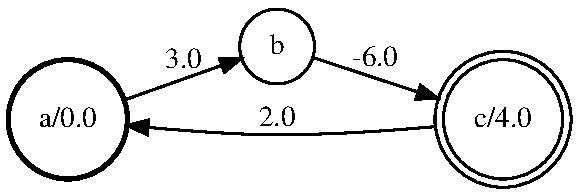
\includegraphics[scale=0.6]{images/fsm1.pdf}
    \captionsetup{singlelinecheck=off}
    \caption[example/fsm1]{example of FSM in the log-semiring where:
    \begin{align}
        Q &= \{1, 2, 3\} & \Sigma &= \{a, \dots, z\} \\
        \boldsymbol{\alpha} &= \begin{bmatrix}
            0 \\
            -\infty \\
            -\infty
        \end{bmatrix} &
        \boldsymbol{\omega} &= \begin{bmatrix}
            -\infty \\
            -\infty \\
            4
        \end{bmatrix} \\
        \mathbf{T} &= \begin{bmatrix}
            -\infty & 3 & -\infty \\
            -\infty & -\infty & -6 \\
            2 & -\infty & -\infty
        \end{bmatrix} &
        \boldsymbol{\lambda} &= \begin{bmatrix}
            a \\
            b \\
            c
        \end{bmatrix}
    \end{align}}
    \label{fsm:fig:example1}
\end{figure}

\paragraph{input sequence:} We define an input sequence $\mathbf{s}$ to
a FSM as a sequence of labels:
\begin{align}
    \mathbf{s} = \prod_{i=1}^n s_i, \quad s_i \in L.
\end{align}
The weight of an input sequence is given by the function
$\nu: L \rightarrow K$:
\begin{align}
    \nu(\mathbf{s}) = \sum_{ \mathbf{x} \in P} \mu(\mathbf{x}),
\end{align}
where $P = \{\boldsymbol{\pi} : \; \sigma(\boldsymbol{\pi}) = \mathbf{s}, \;
\boldsymbol{\pi} \in \mathcal{M} \}$ is the set of paths from
$\mathcal{M}$ with label sequence $\mathbf{s}$.
We say that an input sequence is \emph{accepted by $\mathcal{M}$} if
$\nu(\mathbf{s}) > 0$. We denote $S$ the set of accepted input sequence
of a FSM, i.e. $S = \{\mathbf{s} : \nu(\mathbf{s}) > 0 \}$.

\subsection{Total sum}

We define the total weight sum of a FSM $\zeta$ as the sum of all the
weights of its accepted input sequences:
\begin{align}
    \zeta = \sum_{\mathbf{s} \in S} \nu(\mathbf{s}).
\end{align}
The total weight sum can be estimated efficiently via dynamic
programming. Let be $\zeta_n$ the \emph{partial total sum} of a FSM
$\mathcal{M}$ defined as the sum of all the weights of accepted input
sequence of size smaller of equal to $n$:
\begin{align}
    \zeta_n = \sum_{\mathbf{s} \in
        \{ \mathbf{s} : \; | \mathbf{s} | \le n, \; \mathbf{s} \in S \}}
        \nu(\mathbf{s}).
\end{align}
$\zeta_n$ can be calculated through the following recursion:
\begin{align}
    \mathbf{v}_n &= \mathbf{T}^\top \mathbf{v}_{n-1} \\
    \zeta_n &= \boldsymbol{\omega}^\top \mathbf{v}_n,
\end{align}
where the recursion is initialized with $\mathbf{v}_1 = \boldsymbol{\alpha}$

